%
% This is the LaTeX template file for lecture notes for EE 382C/EE 361C.
%
% To familiarize yourself with this template, the body contains
% some examples of its use.  Look them over.  Then you can
% run LaTeX on this file.  After you have LaTeXed this file then
% you can look over the result either by printing it out with
% dvips or using xdvi.
%
% This template is based on the template for Prof. Sinclair's CS 270.

\documentclass[twoside]{article}
\usepackage{graphicx}
\usepackage{algorithm}
\usepackage{algpseudocode}
\usepackage{graphics}
\setlength{\oddsidemargin}{0.25 in}
\setlength{\evensidemargin}{-0.25 in}
\setlength{\topmargin}{-0.6 in}
\setlength{\textwidth}{6.5 in}
\setlength{\textheight}{8.5 in}
\setlength{\headsep}{0.75 in}
\setlength{\parindent}{0 in}
\setlength{\parskip}{0.1 in}

%
% The following commands set up the lecnum (lecture number)
% counter and make various numbering schemes work relative
% to the lecture number.
%
\newcounter{lecnum}
\renewcommand{\thepage}{\thelecnum-\arabic{page}}
\renewcommand{\thesection}{\thelecnum.\arabic{section}}
\renewcommand{\theequation}{\thelecnum.\arabic{equation}}
\renewcommand{\thefigure}{\thelecnum.\arabic{figure}}
\renewcommand{\thetable}{\thelecnum.\arabic{table}}

%
% The following macro is used to generate the header.
%
\newcommand{\lecture}[4]{
   \pagestyle{myheadings}
   \thispagestyle{plain}
   \newpage
   \setcounter{lecnum}{#1}
   \setcounter{page}{1}
   \noindent
   \begin{center}
   \framebox{
      \vbox{\vspace{2mm}
    \hbox to 6.28in { {\bf EE 382C/361C: Multicore Computing
                        \hfill Fall 2016} }
       \vspace{4mm}
       \hbox to 6.28in { {\Large \hfill Lecture #1: #2  \hfill} }
       \vspace{2mm}
       \hbox to 6.28in { {\it Lecturer: #3 \hfill Scribe: #4} }
      \vspace{2mm}}
   }
   \end{center}
   \markboth{Lecture #1: #2}{Lecture #1: #2}
   %{\bf Disclaimer}: {\it These notes have not been subjected to the
   %usual scrutiny reserved for formal publications.  They may be distributed
   %outside this class only with the permission of the Instructor.}
   \vspace*{4mm}
}

%
% Convention for citations is authors' initials followed by the year.
% For example, to cite a paper by Leighton and Maggs you would type
% \cite{LM89}, and to cite a paper by Strassen you would type \cite{S69}.
% (To avoid bibliography problems, for now we redefine the \cite command.)
% Also commands that create a suitable format for the reference list.
\renewcommand{\cite}[1]{[#1]}
\def\beginrefs{\begin{list}%
        {[\arabic{equation}]}{\usecounter{equation}
         \setlength{\leftmargin}{2.0truecm}\setlength{\labelsep}{0.4truecm}%
         \setlength{\labelwidth}{1.6truecm}}}
\def\endrefs{\end{list}}
\def\bibentry#1{\item[\hbox{[#1]}]}

%Use this command for a figure; it puts a figure in wherever you want it.
%usage: \fig{NUMBER}{SPACE-IN-INCHES}{CAPTION}
\newcommand{\fig}[3]{
			\vspace{#2}
			\begin{center}
			Figure \thelecnum.#1:~#3
			\end{center}
	}
% Use these for theorems, lemmas, proofs, etc.
\newtheorem{theorem}{Theorem}[lecnum]
\newtheorem{lemma}[theorem]{Lemma}
\newtheorem{proposition}[theorem]{Proposition}
\newtheorem{claim}[theorem]{Claim}
\newtheorem{corollary}[theorem]{Corollary}
\newtheorem{definition}[theorem]{Definition}
\newenvironment{proof}{{\bf Proof:}}{\hfill\rule{2mm}{2mm}}

% **** IF YOU WANT TO DEFINE ADDITIONAL MACROS FOR YOURSELF, PUT THEM HERE:

\begin{document}
%FILL IN THE RIGHT INFO.
%\lecture{**LECTURE-NUMBER**}{**DATE**}{**LECTURER**}{**SCRIBE**}
\lecture{3}{September 1}{Vijay Garg}{Travis Brannen}
%\footnotetext{These notes are partially based on those of Nigel Mansell.}

% **** YOUR NOTES GO HERE:

% Some general latex examples and examples making use of the
% macros follow.  
%**** IN GENERAL, BE BRIEF. LONG SCRIBE NOTES, NO MATTER HOW WELL WRITTEN,
%**** ARE NEVER READ BY ANYBODY.
\section{Introduction}

This class centered around analysis of various methods to achieve mutual exclusion in a concurrent environment.  First, we review the proof of Peterson's Algorithm from last time.  Next, we extend Peterson's so that it can be used for more than two processes ultimately arriving a tthe Filter Algorithm.  We then briefly cover another extension of Peterson's algorithm, the so called Tournament.  We briefly discuss the issue of multiwriter variables.  Finally, we discuss another algorithm for concurrent mutual exclusion, the Bakery algorithm.

\section{Peterson's Algorithm}
Previously we developed Peterson's algorithm, and java code for the algorithm can be found in [1].  We also added, for the purpose of our proof, the boolean array $trying$.  Here is PetersonAlgorithm.java with the variable $trying$:
\begin{verbatim}
class PetersonAlgorithm implements Lock {
    boolean wantCS[] = {false, false};
    boolean trying[] = {false, false};
    int turn = 1;
    public void requestCS(int i) {
        int j = 1 - i;
        trying[i] = true;
        wantCS[i] = true;
        turn = j;
        while (wantCS[j] && (turn == j)) ;
        trying[i] = false;
        // process i enters critical section after returning from this method
    }
    public void releaseCS(int i) {
        // process i leaves critical section upon setting wantCS[i] to false
        wantCS[i] = false;
    }
}
\end{verbatim}

We review the proof for mutual exclusion that takes advantage of $trying$:

Consider predicate H(0), where:
\[H(0) \equiv wantCS[0] \wedge [(turn == 1) \vee ((turn == 0) \wedge trying[1])]\]
\[H(1) \equiv wantCS[1] \wedge [(turn == 0) \vee ((turn == 1) \wedge trying[0])]\]

$P_0$ makes $H(0)$ true just before entering the while loop by setting $turn$=1.
$P_1$ makes $H(1)$ true just before entering the while loop by setting $turn$=0.

$P_1$ cannot falsify $H(0)$.
\begin{itemize}
  \item Only $P_0$ can change the value of $wantCS$[0].
  \item Additionally, 
\[H(0) \Rightarrow turn==1 \vee (turn==0 \wedge (trying[1]))\]
Moving line by line through $requestCS$(1), one can see that although $P_1$ can change $trying$[1] and $turn$, $turn$ is only equal to 0 while $trying$[1] is true. From symmetry, $P_1$ also cannot falsify $H(0)$.
\end{itemize}

Now, we will use the above in our proof of mutual exclusion by contradiction.  First we suppose that both $P_0$ and $P_1$ are in their critical section, a violation of mutual exclusion.  For this to be true, $trying$=\{$false$, $false$\} since both processes have returned from $requestCS$.  Also, $H(0)$ and $H(1)$ are true since both processes made their corresponding predicate true before entering the while loop and the predicates were not made false by any process since then.  Therefore,

\[Both In Critical Section \equiv \neg trying[0] \wedge H(0) \wedge \neg trying[1] \wedge H(1)\Rightarrow turn == 0 \wedge turn == 1\Rightarrow false\]

/section{Filter Algorithms}
Now we try to extend Peterson's Algorithm so that it can be used for N concurrent processes.  To do so, we get rid of the $turn$ variable and replace it with a variable called $last$.  This is to eliminate the need for processes to explicitly reference other processes in their code.

Pseudocode for PetersonN base algorithm:
\begin{verbatim}
wantCS[i] = true
last = i
while( (exists j such that j!=i and wantCS[j]) and last==i )
***CRITICAL SECTION***
wantCS[i] = false
\end{verbatim}

This is very similar to Peterson's algorithm, but close analysis reveals that it will allow N-1 processes to enter the critical section.  However, running N-1 of these "gates" in series allows us to go from N processes, to N-1, to N-2, and so on until only one process exits the filter to enter the critical section at a time.  This gives us an algorithm to enforce mutual exclusion among N processes such that only 1 process enters the critical section at a time.  See PetersonN.java for an implementation of this algorithm[1].  

There are two new variables used in this algorithm.  $gate$ is an array with N integers, with the $i$th position representing the gate $P_i$ is currently waiting behind.  $last$ is an array of integers with the value for last for each gate.  Since we only need N-1 gates, the 0 position of $last$ will be unused.  Also, $gate$[i]=0 indicates that $P_i$ is not currently attempting to access the critical section.

This algorithm may also be modified to allow any number of processes between N-1 and 1 into the critical section, for resources that may be shared between a limited number of users.

Space Complexity: O($N$)
Time Complexity: O($N^2$)

\section{Tournament}
The nested for loops in PetersonN.java mean that it is not very temporally efficient.  Using a tournament structure as shown below would take less time.  Each process would enter a Peterson's Algorithm lock competing with one other process at the bottom.  The winner would compete with the winner of an adjacent contest and so on.  After passing through $log_2$(N) such locks, one process would enter the critical section at a time.
\begin{figure}[h]
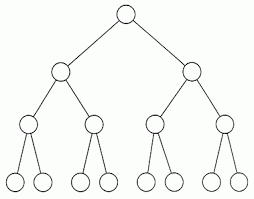
\includegraphics[scale=.5]{binarytree}
\centering
\end{figure}
\section{Multwriter Variables}
SRSW - Single reader single writer\newline
MRSW - Multireader single writer\newline
MRMW - Multireader Multiwriter\newline\newline
SRSW does not pose a concurrency problem.  MRSW allows for sequential consistency but locks are required for strict consistency.  MRMW is the most difficult to implement since without locks even sequential consistency cannot be relied on.
\section{Bakery}
The Bakery Algorithm is another method of locking a shared resource so that only 1 of N processes may use it at once.  The basic idea is that there are two steps to acquiring the lock.  First, you come in through the "doorway" of the bakery and take a number.  This number should be one higher than everyone who is already inside the bakery.  Second, you wait until your number is the lowest number of anyone inside the bakery.  Because of concurrency, it is possible that two processes will enter the bakery simultaneously and get the same number.  Because of this, sequential, persistent process IDs from 0 to N-1 are issued to each process and in the case where two processes have the same number the one with the lower process ID enters the critical section first.

A full java implementation is given in Bakery.java[1].  There are two variables of interest $choosing$ and $number$.  $P_i$ sets $choosing[i]$ to true when it enters the doorway and to false once it has a $number$.  The $choosing$ variable allows a process to ensure that any other processes that were choosing while it was choosing have finished by the time it attempts to enter the critical section.  $number[i]$ is set by $P_i$ in the doorway to be equal to $max(number)$ + 1 and used to determine who should get in to the critical section.  $number$ is initialized to an array of all zeros because zero is used as a flag indicating that a process is not attempting to enter the critical section.  Also for this reason, $number[i]$ is set to 0 after $P_i$ exits the critical section.

Note that in the for loop checking if a process has the smallest number you need not explicitly take care of the case where j=i since the while condition will always return false in this case.

{\bf Check for Mutual Exclusion}\\
If $P_i$ is in the critical section and $P_k$ (s.t. k!=i) has already chosen its number, then $(number[i], i) < (number[k], k)$.  Then, assume $P_i$ and $P_k$ are in the critical section.  This is a contradiction by the following:

t=time when $P_i$ checked $choosing[k]$ and found it false.
\begin{figure}[h]
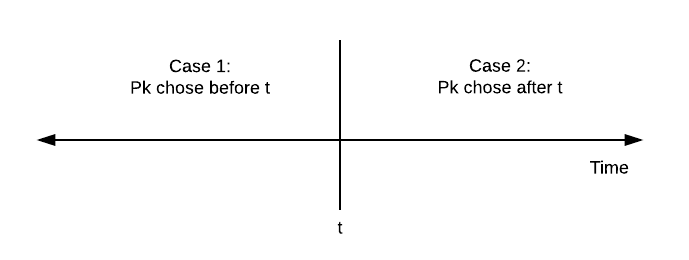
\includegraphics[scale=.5]{bakeryprooffig1}
\centering
\end{figure}

In both Case 1 and Case 2, $(number[i], i) < (number[k], k)$.

\section{Final Thoughts}
In Java, even with locking algorithms you can still have mutual exclusion.  This is because by default sequential consistency is not enforced.  Multiple copies of variables are stored by main memory and the caches for each processor.  You can use the volatile keyword for variables and the synchronized keyword for functions to enforce sequential consistency.  The atomic keyword for variables can also be used to implement test and set.

\section*{References}
\beginrefs
\bibentry{1} https://github.com/vijaygarg1/UT-Garg-EE382C-EE361C-Multicore/tree/master/chapter1-threads
\endrefs


\end{document}

